\documentclass{article}

\usepackage{amsmath, amsthm, amssymb,amsfonts}
\usepackage{fullpage}
\usepackage{tabu}
\usepackage{graphicx,float,wrapfig}
\usepackage{caption}

\providecommand{\e}[1]{\ensuremath{\times 10^{#1}}}

\begin{document}

\title{Problem with SmolDyn Conversion}
\author{Shawn Garbett}

\section{Introduction}

A basic enzymatic reaction is explored as a proof of concept.

\begin{equation}
S + E \overset{k_1}{\underset{k_{-1}}{\rightleftarrows}} C \overset{k_2}{\rightarrow} P + E
\end{equation}

with $k_1 = 0.05 \mu M^{-1} s^{-1}$, $k_{-1} = 5.0 s^{-1}$, $k_2 = 1.0 s^{-1}$, $S_{init} = 100 \mu M$, and $E_{init} = 50\mu M$.

Running this as a straight forward ODE solution is easily done, treating the initial values as molarity concentrations. The question becomes translation of reaction rates and size of space to maintain the numbers as copy numbers in Smoldyn.

\section{Smoldyn Conversion}

\subsection{Size}

To keep the $100\mu M$ concentration with a copy number of 100 requires setting the environment size. Smoldyn is unitless, but assumes that one is specifying in terms of some unit length and volume. The default unit length is ``pixels'', or a convenient equivalent $10 nm$. So one cubic voxel, $px^3$ is equal to $1000 nm^3$. However, for this right now I will keep the units in $px$.

\begin{center}
\begin{tabular}{c|c}
$100 \mu M$ & 6.022045\e{-3} $px^{-3}$\\
\hline
 & $10 \mu M$ \\
\end{tabular} = 6.022045\e{-2} / $px^3$
\end{center}

Now to compute size required for 100 molecules using this.


\begin{equation}
\frac{100}{L^3} = 6.022045\e{-2} / px^3
\end{equation}
\begin{equation}
    L = 11.84183
\end{equation}

So for 100 molecules, a width in pixels in Smoldyn is approximately 12 pixels to a side preserves the $100\mu M$ concentration, this corresponds to a volume of $1.660565\e{6} nm^3$.

\subsection{Bimolecular Reactions}

The unimolecular reactions remain constant. The $k_1$ constant needs adjusting to due to its biomolecularity. 

\begin{center}
\begin{tabular}{c|c|c|c}
0.05 $\mu M^{-1} s^{-1}$ &  $1\e{6} M^{-1}$ & 0.1660565 $px^3 ms^{-1 }$ & 1000 $ms$\\
\hline
 & $1 \mu M^{-1}$ & $10^5 M^{-1} s^{-1}$ & 1 $s$ \\
\end{tabular} = 83.028 $px^3 s^{-1}$ 
\end{center}

This works, but only with diffusion coefficients sufficiently high. Right now, I'm using $100 px^2 s^{-1}$ and the following results:

\begin{figure}[h]
\centering
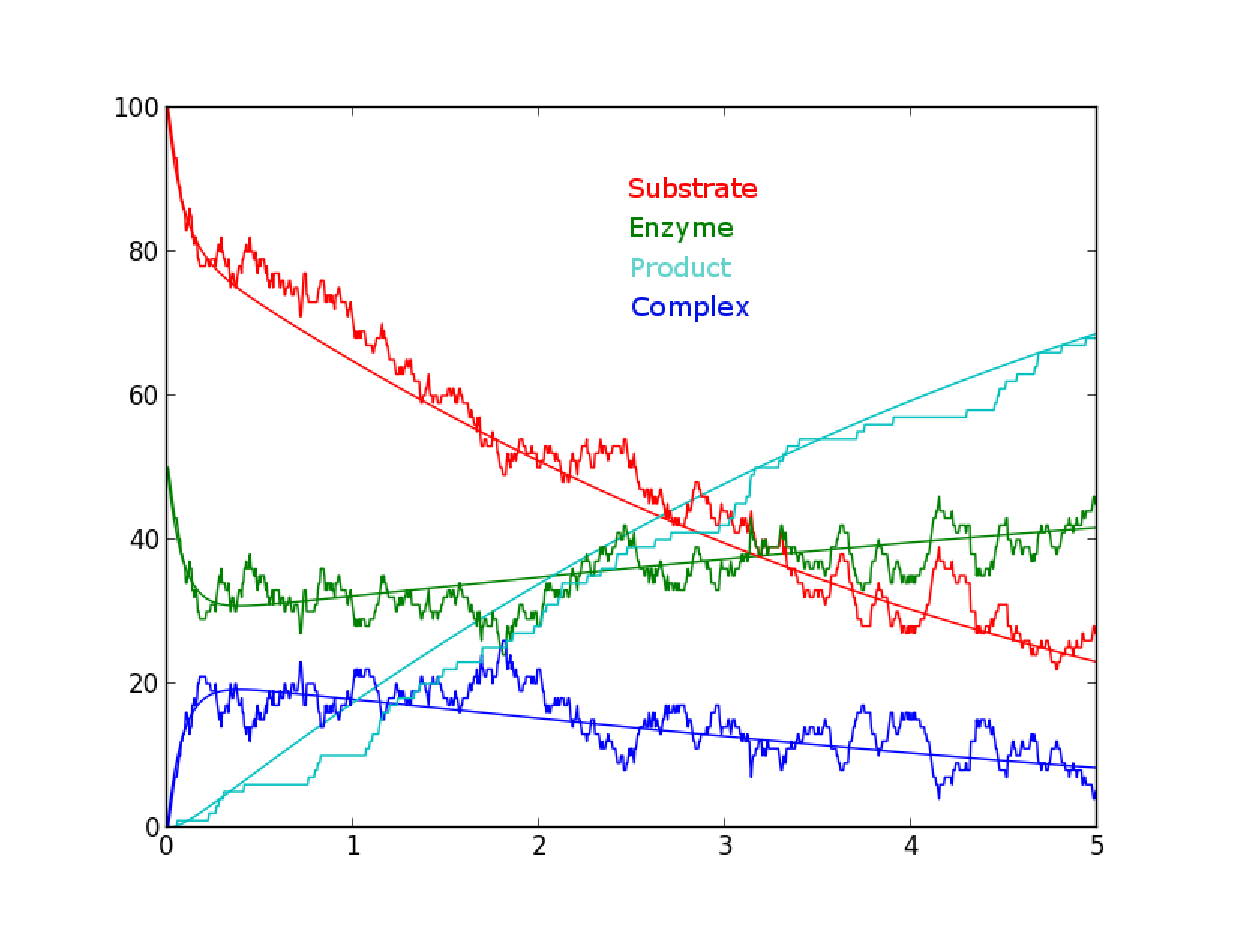
\includegraphics[width=16cm, height=12cm]{figure_1.eps}
\caption{5 Second Simulation ODE vs. Smoldyn, $k_1=83.028$}
\label{fig1}
\end{figure}


\end{document}